\section{The Queue Transmission Model (QTM)}


\begin{figure*}[t]
\centering
%  trim={<left> <lower> <right> <upper>}
\subfigure[]{
\label{subfig:overlay}
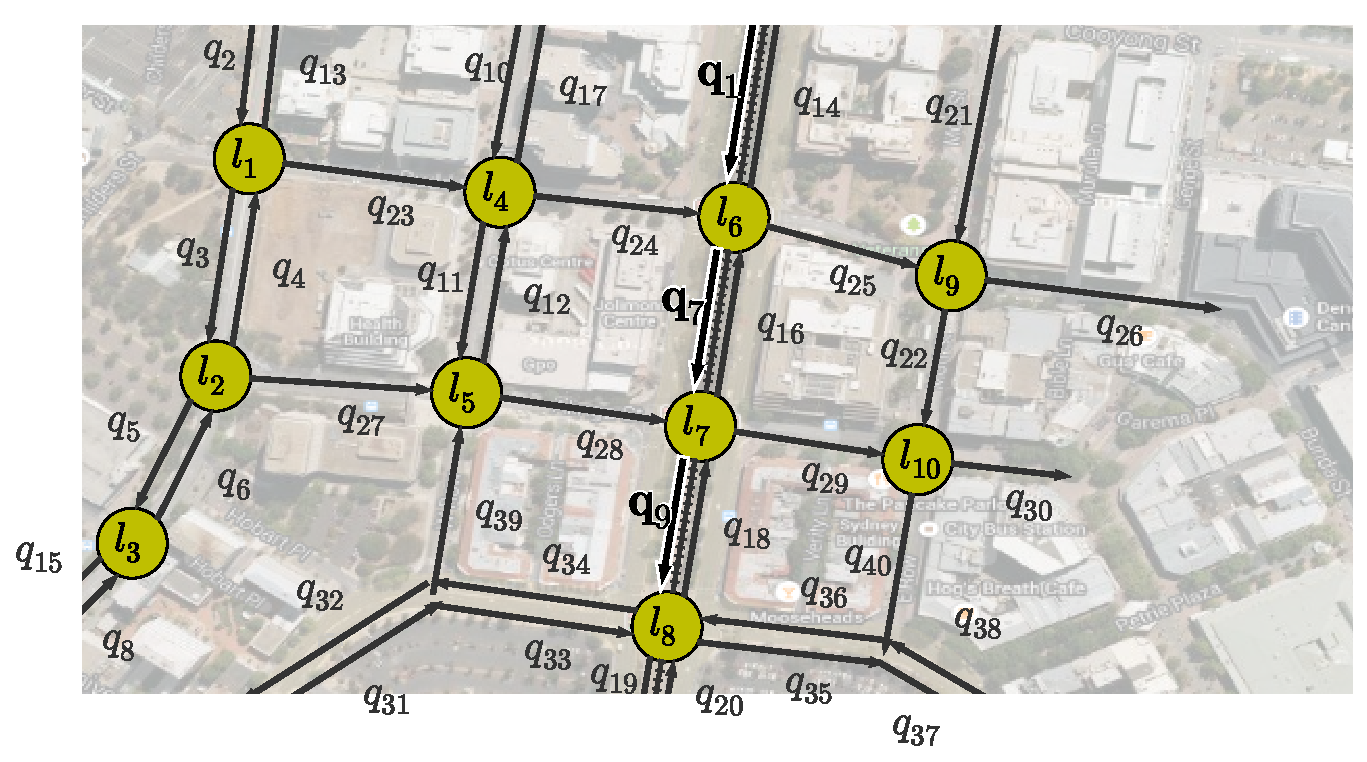
\includegraphics[width=0.5\textwidth,trim={1.3cm 1.2cm 3cm 0.5cm},clip]{canberra_transit.pdf}}
\subfigure[]{
\label{subfig:example}
%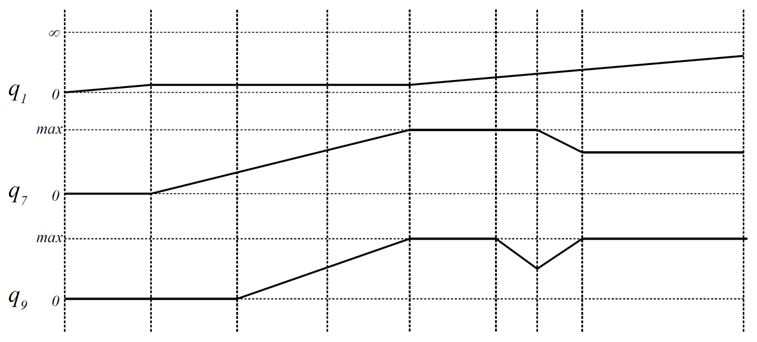
\includegraphics[width=0.45\textwidth,trim={0cm 0cm 0cm 0cm},clip]{map_example.png}
\hspace{-3mm}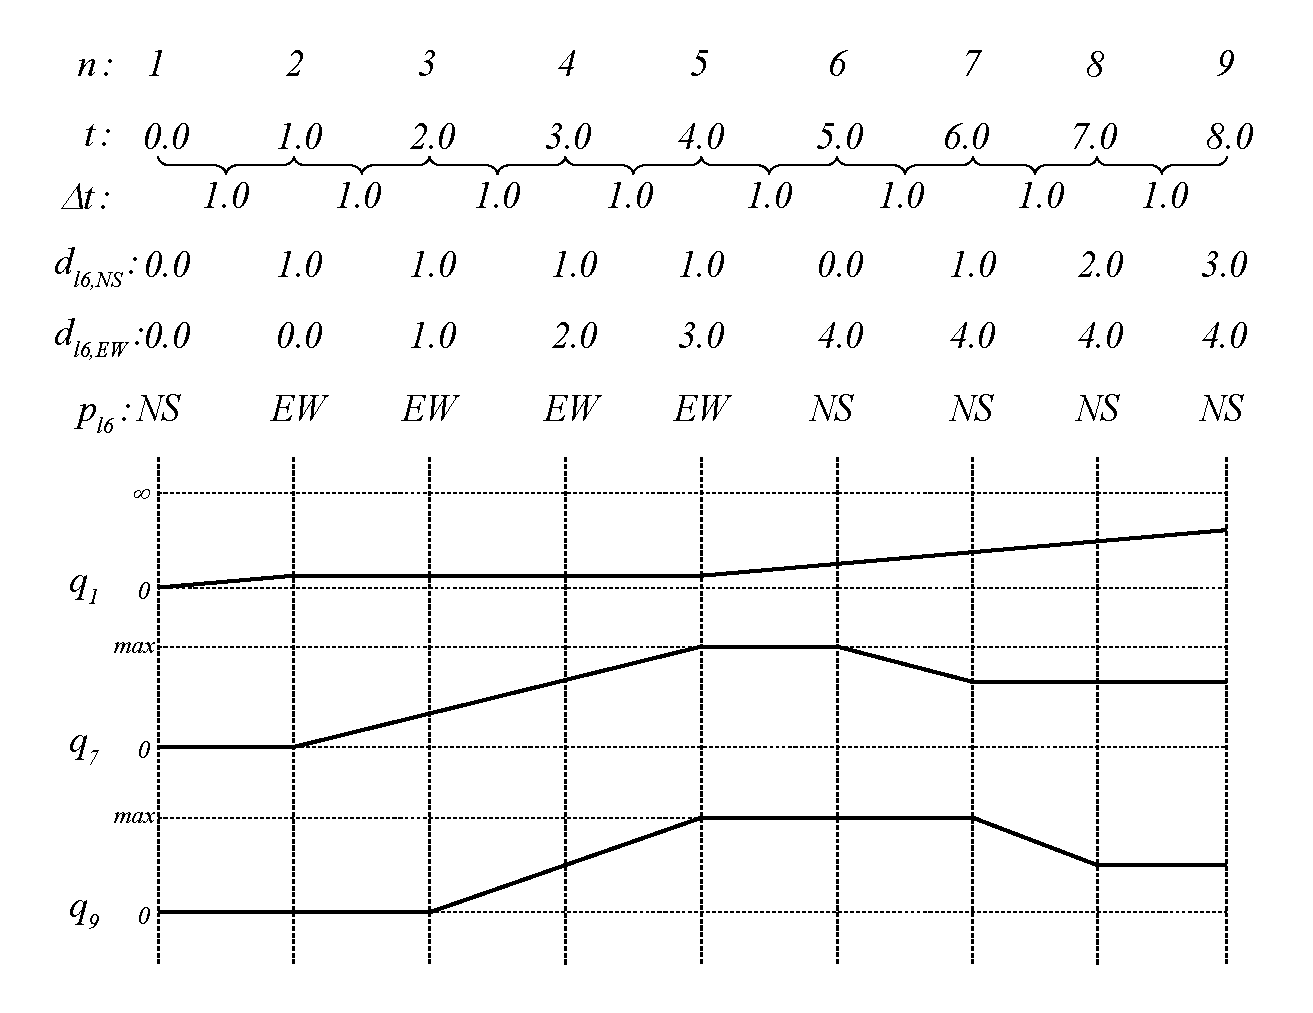
\includegraphics[width=0.44\textwidth,trim={0cm 0cm 0cm 0cm},clip]{pw_queues_homogenous.pdf}
\vspace{-2mm}
}
% NOTE: Reviewers like to skim a paper by reading captions so I intentionally
\caption{(a) Example of a real traffic network with a central light rail modeled
  using the
  QTM. (b) \Omit{A preview of different QTM model parameters as a function
  of discretized time intervals.}
  A preview of different QTM model parameters as a function
  of discretized time intervals indexed by $n$.
  For each $n$, we show the following parameters: the elapsed time
  $t$, the time step length $\Delta t$, the cumulative
  duration $d$ of two different light phases for $l_6$, the phase $p$
  of light $l_6$, and the traffic volume of different queues $q$
  linearly interpolated between time points.  There is technically a
  binary $p$ for each phase, but we abuse notation and simply
  show the current active phase: $\mathit{NS}$ for \emph{north-south green} and 
  $\mathit{EW}$ for \emph{east-west green} assuming the top of the map is north.
  Here we see that traffic progresses from $q_1$ to $q_7$ to $q_9$
  according to light phases and traffic propagation delay.
  %Time interval boundaries are only necessary at
  %nonlinear changepoints in queue volume.
  We refer to the QTM model section for
  precise notation and technical definitions.}
\label{fig:qtm}
%
\end{figure*}


%% TODO(fwt): We need to say that we handle expected number of cars instead of
%% physical cars, so its fine to have fractions of cars.

To investigate the impact of light rail schedules on conventional
traffic networks we need a model of both traffic flow and light rail
constraints.  As a model of traffic flow, we define the Queue
Transmission Model (QTM)~\cite{guilliard2016trb}.  Informally, we show an example of a traffic
network and the evolution of the variables in a QTM model over time
in Figure~\ref{fig:qtm}.  Formally a QTM is a tuple $(\Qset, \Lset,
\vecDT, \MatQIN)$, where \Qset and \Lset are, respectively, the set of
queues and lights;
%
\vecDT is a vector of size \Nn representing the discretization of the problem
horizon $[0,\TMAX]$ and the duration in seconds of the $n$-th
time interval is denoted as \DT[n];
%
%%
%% TODO(fwt): Maybe mention that car that are denied entry could be stored in a
%% infinity capacity queue and eventually be allowed to enter the network. Also
%% point out that this case doesn't happen in our experiments
%%
%% TODO(fwt): Maybe mention that add \QIN{i} can estimate through a model
%% learned from historical data.
%
and \MatQIN is a matrix $|\Qset| \times \TMAX$ in which \QIN{i}{n} represents
the flow of cars requesting to enter queue $i$ from the outside of the network
at time $n$.



A \textbf{traffic light} $\tl \in \Lset$ is defined as the tuple $(\CTMIN{\tl},
\CTMAX{\tl},$ $\Pset_\tl, \VecPTMIN{\tl}, \VecPTMAX{\tl})$, where:
%
\begin{itemize}
%
\item $\Pset_\tl$ is the set of phases of $\tl$;
%
\item \CTMIN{\tl} (\CTMAX{\tl}) is the minimum (maximum) allowed cycle time for
\tl; and
%
\item \VecPTMIN{\tl} (\VecPTMAX{\tl}) is a vector of size $|\Pset_\tl|$ and
  \PTMIN{\tl}{k} (\PTMAX{\tl}{k}) is the minimum (maximum) allowed time for
  phase $k \in \Pset_\tl$. 
%
\end{itemize}


A \textbf{queue} $i \in \Qset$ represents a segment of road that vehicles
traverse at free flow speed; once traversed, the vehicles are vertically stacked
in a stop line queue.
% of maximum capacity \QMAX{i}.
%
Formally, a queue~$i$ is defined by the tuple~$(\QMAX{i}, \QDELAY{i}, \QOUT{i},
\Fvec_i, \Prvec_i, \QPset{i})$ where:
%
\begin{itemize}
%
%% TODO(fwt): clarify that this is the capacity of stop line queue
\item \QMAX{i} is the maximum capacity of $i$;
%
\item \QDELAY{i} is the time required to traverse $i$ and reach the stop line;
%
\item \QOUT{i} represents the maximum traffic flow from $i$ to the outside of
  the modeled network;
%
\item $\Fvec_i$ and $\Prvec_i$ are vectors of size \Qn and their $j$-th entry
  (i.e., \FMAX{i}{j} and \FTURN{i}{j}) represent the maximum flow from queue $i$
  to $j$ and the turn probability from $i$ to $j$ ($\sum_{j \in
  \Qset}\FTURN{i}{j} = 1$), respectively; and
%
\item \QPset{i} denotes the set of traffic light phases controlling the outflow
  of queue $i$.
%
\end{itemize}

%
%% TODO(fwt): Not sure if still need to talk about CTM or simply say 
%
%Differently than the CTM \cite{daganzo1994cell,lin2004enhanced}, the QTM does
%not assume that $\DT[n] = \QDELAY{i}$ for all $n$ and $i$.
%
For this work, we assume that \QDELAY{i} is divisible by every different value
of $\DT[n]$.
%
This allow us to have queues with different travel time at free flow speed
resulting in a non-first order Markovian model as explained in next section.

%that is, the QTM can represent non-homogeneous time intervals.
%%
%%%(\cref{subfig:example}).
%%
%The only requirement over \DT[n] is that no traffic light maximum phase time is
%smaller than any \DT[n] since phase changes occur only between time intervals;
%formally, $\DT[n] \le \min_{\tl \in \Lset, k \in \Pset_\tl} \PTMAX{\tl}{k}$ for
%all $n \in \{1,\dots,\Nn\}$.
%
% TODO \toIain{Maybe bring forward a small network and any other figure that
% would help illustrate the model and comment about it.}



\subsection{Computing Traffic Flows with QTM}

In this section, we present how to compute traffic flows using QTM.
%and \authorHighlight{non-homogeneous time intervals \DT[]}.
%
We assume for the remainder of this section that a \emph{valid} control plan for
all traffic lights is fixed and given as parameter;
%
formally, for all $\tl \in \Lset$, $k \in \Pset_\tl$, and interval $n \in
\{1,\dots,N\}$, the binary variable $\p{\tl}{k}$ is known a priori and indicates
if phase $k$ of light \tl is active~(i.e., $\p{\tl}{k} = 1$) or not on interval
$n$.


We represent the problem of finding the maximal flow between
capacity-constrained queues as a Linear Program~(LP) over the following
variables defined for all interval $n \in \{1,\dots,\Nn\}$ and queues $i$ and
$j$:
%
\begin{itemize}
%
\item $\q{i} \in [0,\QMAX{i}]$, traffic volume waiting in the stop line of queue
  $i$ at the beginning of interval~$n$;
%
\item $\inq{i} \in [0,\QIN{i}{n}]$, inflow to the network via queue $i$ during
  interval $n$;
%
\item $\outq{i} \in [0,\QOUT{i}]$, outflow from the network via queue $i$ during
  interval $n$; and
%
\item $\f{i}{j} \in [0,\FMAX{i}{j}]$, flow from queue $i$ into queue $j$ during
  interval $n$.
%
\end{itemize}



%% FWT: These constraints are not necessary because we defined the domain of the
%% variables in the paragraph above
%\inq{i} &\le \QIN{i}{n} \tag{C1}\label{eq:C1}\\ 
%\outq{i} &\le \QOUT{i} \tag{C2}\label{eq:C2}\\
% \q{i} &\le \QMAX{i} \tag{C9}\label{eq:C9}\\




The maximum traffic flow from queue $i$ to queue $j$ is enforced by
\cref{c:turnProb,c:maxFlow}.
%
\eqref{c:turnProb} ensures that only the fraction $\FTURN{i}{j}$ of the total
internal outflow of $i$ goes to $j$, and \eqref{c:maxFlow} forces the flow from
$i$ to $j$ to be zero if all phases controlling $i$ are inactive.  (i.e.,
$\p{\ell}{k} = 0$ for all $k \in \QPset{i}$).
%
%If more than one phase $\p{\ell}{k}$ is active, then
%\eqref{c:turnProbAndMaxFlow} is subsumed by the domain upper bound of
%$\f{i}{j}$.
%
%\noindent\begin{minipage}{0.5\linewidth}
\begin{cAlign} 
%
\f{i}{j}\!\le\!\FTURN{i}{j}\!\sum_{k=1}^{\Qn}\!\f{i}{k}\tagconstrain{c:turnProb}\\
%
%\end{cAlign}
%%\end{minipage}%
%%\begin{minipage}{0.5\linewidth}
%\begin{cAlign} 
%
\f{i}{j}\!\le\!\FMAX{i}{j}\!\sum^{\phantom{\Qn}}_{\makebox[0pt]{$\scriptstyle
\p{\ell}{k}\!\in\!\QPset{i}$}}\p{\ell}{k}
\tagconstrain{c:maxFlow}
%
\end{cAlign}
%\end{minipage}\par\vspace{\belowdisplayskip}

%\begin{cAlign} 
%%
%\f{i}{j} \le \FTURN{i}{j} \sum_{k=1}^{\Qn} \f{i}{k}
%%\tagconstrain{c:turnProb}\\ \f{i}{j}
%\le \FMAX{i}{j} \sum_{\p{\ell}{k} \in \QPset{i}} {\p{\ell}{k}}
%%\tagconstrain{c:maxFlow}
%\tagconstrain{c:turnProbAndMaxFlow}
%%
%\end{cAlign}




%% TODO(fwt): improve the beginning of this paragraph

To simplify the presentation of the remainder of the LP, we define the helper
variables \qin{i}~\eqref{def:qin} and \qout{i}~\eqref{def:qout} to,
respectively, represent the volume of traffic to enter and leave queue $i$
during interval~$n$, and  $\tn[n] = \sum_{x=1}^{n} \DT[x]$ to represent the time
elapsed since the beginning of the problem until the end of interval \DT[n].
%
%
%\tn[n]~\eqref{def:tn}
%
%
\begin{cAlign}
%
\qin{i} &= \DT (\inq{i} + \Omit{\textstyle} \sum_{j=1}^{\Qn} \f{j}{i}) \tagconstrain{def:qin} \\
%
\qout{i} &= \DT (\outq{i} + \Omit{\textstyle}  \sum_{j=1}^{\Qn} \f{i}{j})
\tagconstrain{def:qout}
%\\
%
%\tn[n] &= \sum_{x=1}^{n} \DT[x] \tagconstrain{def:tn}
%
\end{cAlign}



% Introduce the idea of V_i
In order to account for the case where \QDELAY{i} is larger than \DT[], we need to
find the volume of traffic that entered queue~$i$ between two points
in time $x$ and $y$.
%
This volume of traffic, denoted as $\Vol_i(x,y)$, is obtained by integrating
\qin{i} over $[x,y]$ and is defined in~\eqref{eq:vol} where $T^{-1}(x)$ is the
function that returns $j \in \{0,\dots,N\}$ such that $x$ equals $t_j$ (i.e.,
the $j$-th time step).
%
Since we assumed that \QDELAY{i} is divisible by the different \QDELAY{i},
$T^{-1}(x)$ is always well-defined, i.e., there always exists $j$ such that $x$
equals $t_j$.
%
Because the QTM dynamics are \emph{piecewise linear}, \qin{i} is a step function
w.r.t.~time and this integral reduces to the sum of \qin{i} over the intervals
between $T^{-1}(x)$ and $T^{-1}(y)$.
%
\begin{equation} \label{eq:vol}
%
\Vol_{i}(x,y) = \Omit{\textstyle} \sum_{k=T^{-1}(x)}^{T^{-1}(y)} \qin[k]{i}
%
\end{equation}


Using these helper variables, \eqref{c:qUpdate} represents the flow conservation
principle for queue $i$ where $\Vol_i(\tn[n-1]-\QDELAY{i},\tn[n]-\QDELAY{i})$ is
the volume of cars that reached the stop line during \DT[n].
%
Notice that \eqref{c:qUpdate} represents a non-first order Markovian update
because the update considers the previous $n - T^{-1}(t_{n}-\QDELAY{i})$ time
steps, i.e., the number of $\DT[n]$ spanned in \QDELAY{i}.
%
To ensure that the total volume of traffic traversing $i$ (i.e.,
$\Vol_i(\tn[n] - \QDELAY{i}, \tn[n])$) and waiting at the stop line does not
exceed the capacity of the queue, we apply~\eqref{c:10}.
%
\begin{cAlign}
%
& \q{i} = \q[n\!-\!1]{i} - \qout[n\!-\!1]{i}  + 
\Vol_i(\tn[n\!-\!1]  -  \QDELAY{i}, \tn[n]  -  \QDELAY{i}) \tagconstrain{c:qUpdate}\\
%
& \Vol_i(\tn[n] - \QDELAY{i}, \tn[n]) + \q{i} \le \QMAX{i}
\tagconstrain{c:10}
%
\end{cAlign}


%\begin{figure*}[t!]
%\centering
%%  trim={<left> <lower> <right> <upper>}
%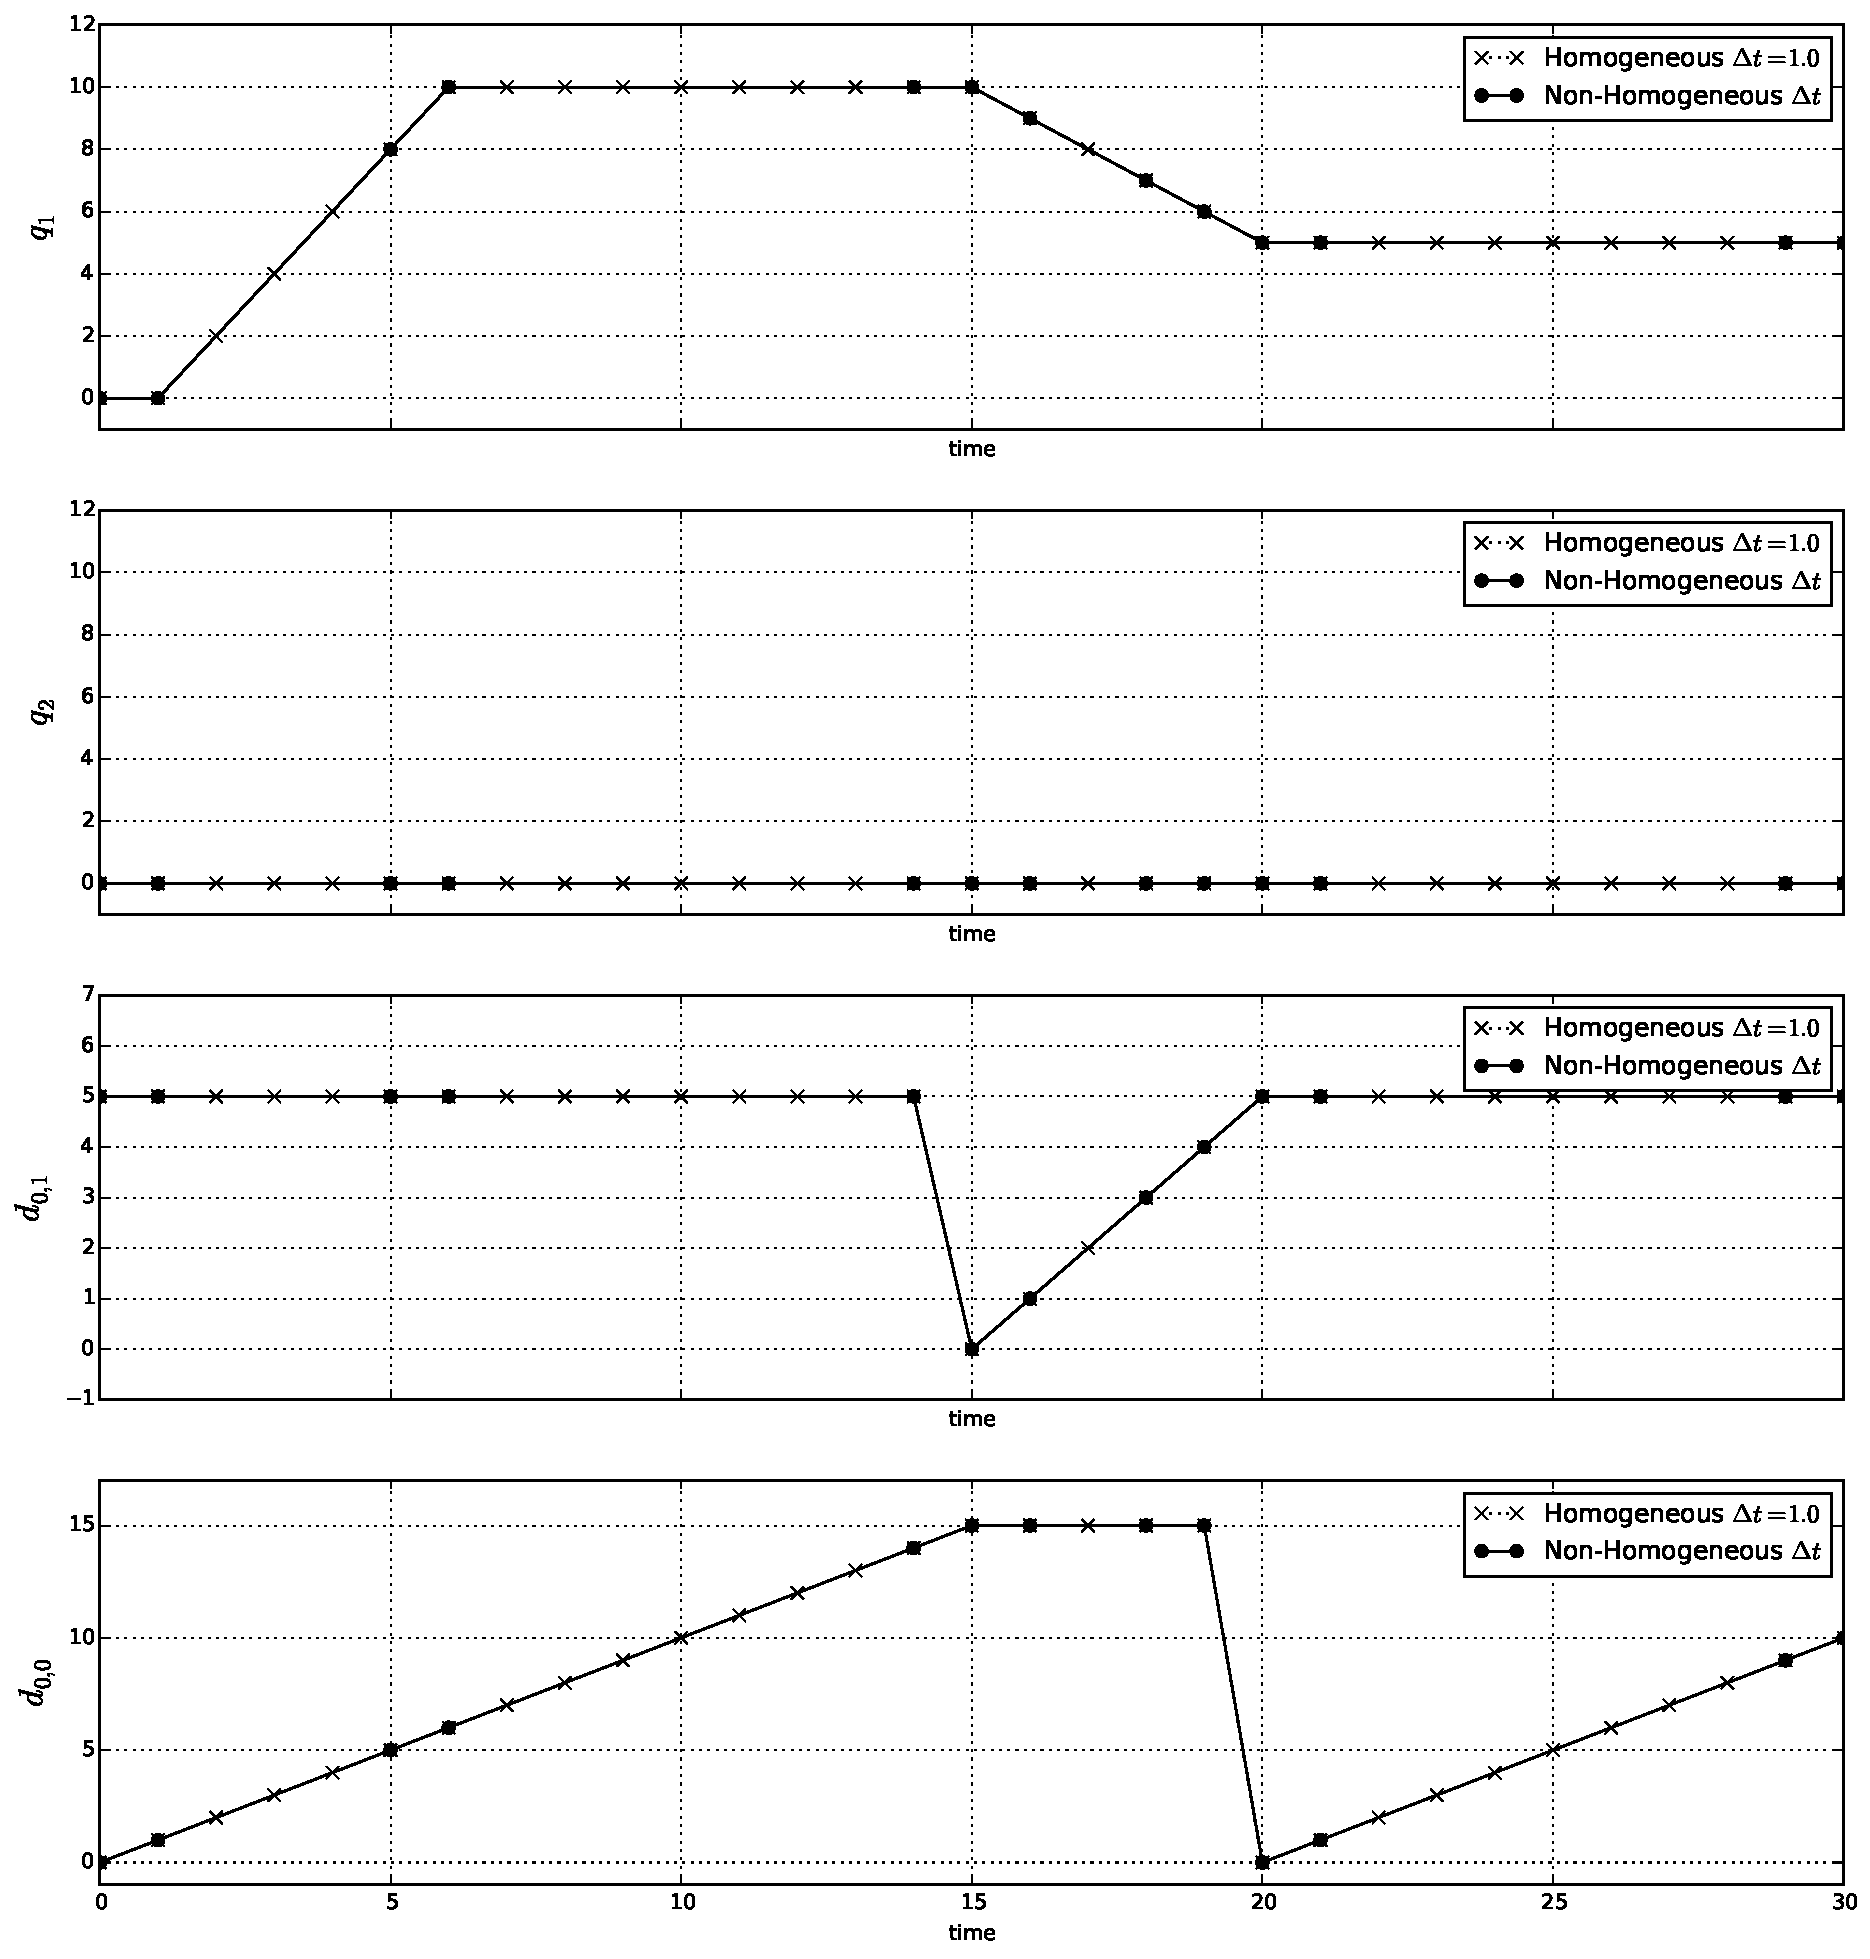
\includegraphics[width=1.0\textwidth,trim={0cm 0cm 0cm 0cm},clip]{convergence_NH.pdf}
%\caption{An example showing the convergence between a homogeneous solution with
%$\Delta t=1.0$ and a non-homogeneous solution over 30 seconds for the same
%network. By using non-homogeneous time steps the same solution is found with
%only 14 sample points compared to 30 for homogeneous solution.}
%\label{fig:converg_c}
%\end{figure*}



As with MILP formulations of CTM (e.g., \trbcite{lin2004enhanced}), QTM is also
susceptible to \emph{withholding traffic}, i.e., the optimizer might prevent
cars from moving from $i$ to $j$ even though the associated traffic phase is
active and $j$ is not full.
%
This might be used by the optimizer to reserve space for traffic from an
alternate queue to further minimize delay in the long-term, even though it leads
to unintuitive traffic flow behavior.
%
We address this well-known issue through our objective
function~\eqref{eq:objFunc} by maximizing the external outflow~\outq{i}
%
%(i.e., both internal and external outflow)
%
and external inflow~\inq{i} of all queues~$i$.
%
This quantity is weighted by the remaining time until the end of the problem
horizon \TMAX to force the optimizer to allow as much traffic volume as possible
into the network and move traffic to the outside of the network as soon as
possible.
%% FWT: not sure if we need to give this extra details
%\trbcite{lin2004enhanced} derive an objective function for the minimisation of
%total delay based on the difference between the cumulative departure and
%arrival curves at the origin and destination. However, such an approach
%requires the network to be cleared at the end of the optimization period.


\begin{equation}
\max 
 \sum_{n=1}^{\Nn} \sum_{i=1}^{\Qn} (\TMAX - \tn + 1) (\outq{i} + \inq{i})
\tag{O1}\label{eq:objFunc}
\end{equation}


%\begin{figure*}[t!]
%\centering
%%  trim={<left> <lower> <right> <upper>}
%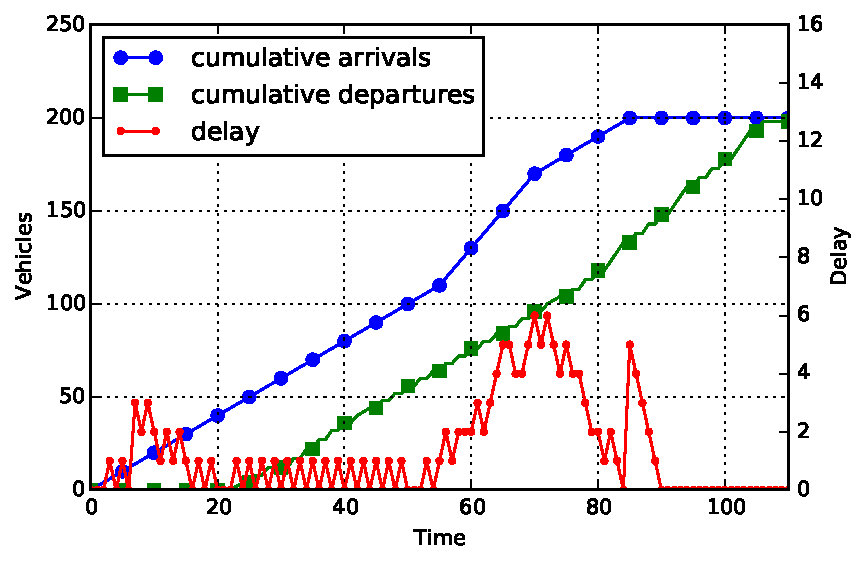
\includegraphics[width=0.55\textwidth,trim={0cm 0cm 0cm 0cm},clip]{cumu_plot_final_6l.pdf}
%\caption{Cumulative arrival (blue) and departure (green) curves, and the
%resulting delay curve (red). The departure curve is maximized by the objective
%function \eqref{eq:objFunc}, which has the same effect as minimizing the area
%under the delay curve.}
%\label{fig:cumu_delay_plot}
%\end{figure*}


The objective \eqref{eq:objFunc} corresponds to minimizing delay in CTM models,
e.g., \eqref{eq:objFunc} is equivalent to the objective function (O3) in
\trbcite{lin2004enhanced} for their parameters
parameters $\alpha = 1$, $\beta = 1$ for the origin cells, and
$\beta = 0$ for all other cells.

%
%
%Figure (fig:cumu-delay-plot) depicts this equivalence using the cumulative
%number of cars entering and leaving a network as a function of time.
%%
%The delay experienced by the vehicles travelling through this network (red curve
%in Figure (fig-cumu-delay-plot) equals the horizontal difference at each point
%between the cumulative departure and arrival curves (less the free flow travel
%time through the network).
%%
%Maximizing \qout{i} weighted by $(\TMAX - \tn +1)$ in \eqref{eq:objFunc} is the
%same as forcing the departure curve to be as close as possible to the arrival
%curve as early as possible; therefore, the area between arrival and departure is
%minimized, which in turn minimizes the delay.



%The objective function~\eqref{eq:objFunc} and
%constraints~(\ref{c:turnProb}--\ref{c:10}) form the LP representing the
%dynamic, piecewise linear model of flow in a QTM network over time when a
%control plan \p{\tl}{k} is given as an input parameter.



%\begin{figure*}[t!]
%\centering
%\subfigure[]{
%\label{subfig:converg_a}
%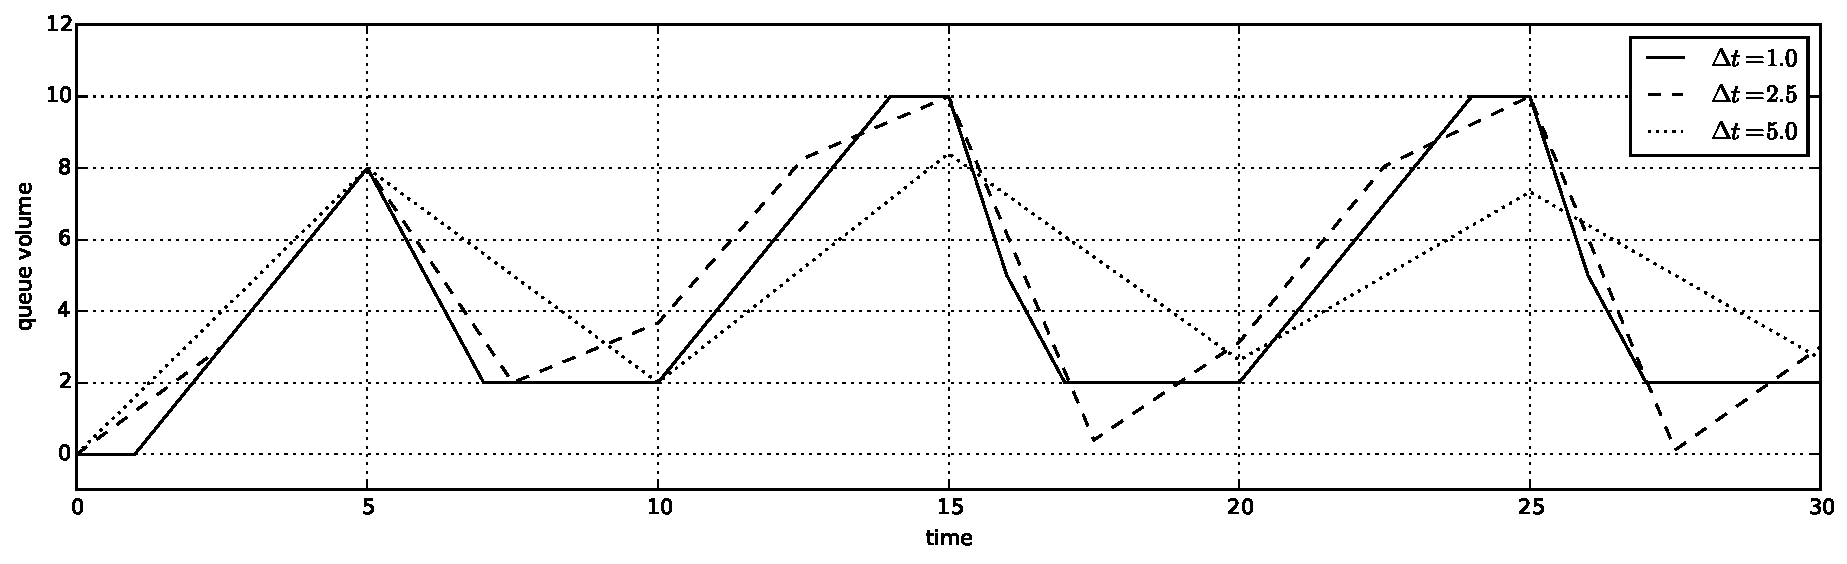
\includegraphics[width=1.0\textwidth,trim={0cm 0cm 0cm 0cm},clip]{convergence.pdf}
%}
%\subfigure[]{
%\label{subfig:converg_b}
%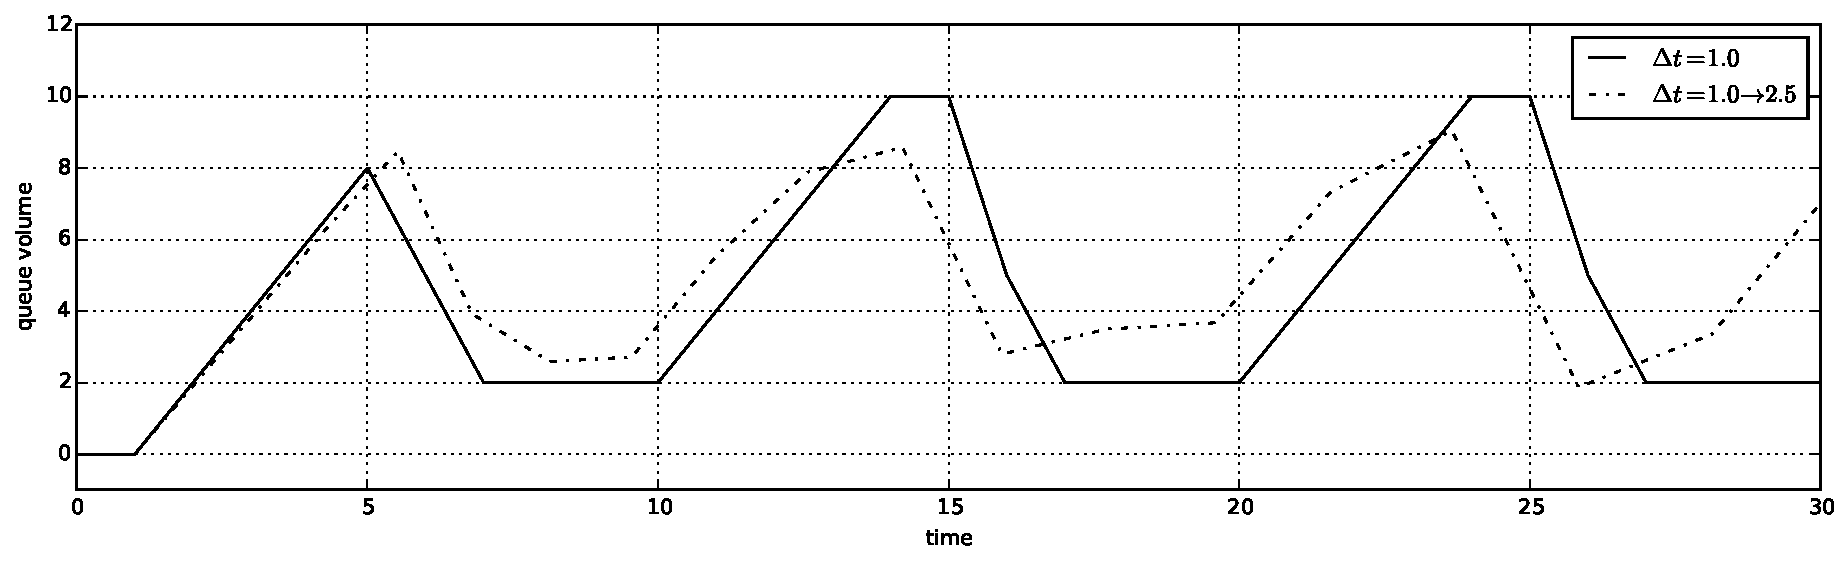
\includegraphics[width=1.0\textwidth,trim={0cm 0cm 0cm 0cm},clip]{convergence_vari.pdf}
%}
%\label{fig:conv}
%%
%\caption{Approximations of a queue volume obtained using homogeneous
%\DT[] = 1s using: (a) homogeneous \DT[] = 2.5s and 5s; and (b) non-homogeneous
%$\DT[n] \approx 0.0956n + 0.9044$ for $n \in \{1,\dots,17\}$.  Here we see
%that (b) achieves accuracy in the near-term that somewhat degrades over
%the long-term, where accuracy will be less critical for receding horizon control.}
%%% Note: would actually be nice to say something about
%%
%\end{figure*}


%To illustrate the representation tradeoff offered by non-homogeneous time
%intervals, we computed flows and queue volumes for a fixed signal control plan
%derived for homogeneous \mbox{\DT[n] = 1s} (ground truth) using different
%discretizations.
%%
%Figure (subfig:converg-a) shows the approximation of the ground truth using
%homogeneous \DT[] = 2.5 and \DT[] = 5.0, and Figure (subfig:converg-b) using
%non-homogeneous time intervals that linearly increases from 1s to 2.5s, i.e.,
%$\DT[n] \approx 0.0956n + 0.9044$ for $n \in \{1,\dots,17\}$.
%%
%As Figure (subfig:converg-a) shows, large time steps can be rough approximations
%of the ground truth.
%%
%Non-homogeneous discretization (Figure (subfig:converg-b)) exploit this fact to
%provide a good approximation in the initial time steps and progressively
%decrease precision for points far in the future.



\section{Traffic Control with MILP-encoded QTM}

In this section, we show how to compute the optimized adaptive control plan by
extending the LP~(\ref{eq:objFunc},~\ref{c:turnProb}--\ref{c:10}) into an
Mixed-Integer LP (MILP).
%
Formally, for all~$\tl \in \Lset$, $k \in \Pset_\tl$, and interval $n \in
\{1,\dots,N\}$, the phase activation parameter~$\p{\tl}{k} \in \{0,1\}$ becomes
a free variable to be optimized.
%
In order to obtain a valid control plan, we enforce that one phase of traffic
light \tl is always active at any interval~$n$~\eqref{c:onlyOnePhaseOn} and
cyclic phase policies where phase changes follow a fixed ordered sequence,
indexed by $k$~\eqref{c:seqPhases}
%
%, i.e., if phase~$k$ was active during interval~$n-1$ and has become inactive
%in interval~$n$, then phase~$k+1$ must be active in interval~$n$.
%
(where \eqref{c:seqPhases} assumes that $k+1$ equals 1 if $k = \Pn{}$).
%
%% TODO: We need to understand this issue better:
% \toIain{I removed the constraint $\p{\ell}{k} + \p{\ell}{k+1} \le 1$ because
% it is subsumed by $\p{\ell}{k} \in \{0,1\}$ and \eqref{c:onlyOnePhaseOn}}
%
%
%% FWT: note sure if the text bellow is necessary
%Note that there could be more than one queue mapped to each $\p[]{\ell}{k}$, or
%their could be none
%
\begin{cAlign}
%
\Omit{\textstyle} \sum_{k=1}^{\Pn} \p{\ell}{k} &=
1\tagconstrain{c:onlyOnePhaseOn}\\
%
\p[n-1]{\ell}{k} &\le \p{\ell}{k} + \p{\ell}{k+1}\tagconstrain{c:seqPhases}
%
\end{cAlign}


%\begin{figure*}[t!]
%\centering
%%  trim={<left> <lower> <right> <upper>}
%\subfigure[]{
%\label{fig:pd:inc}
%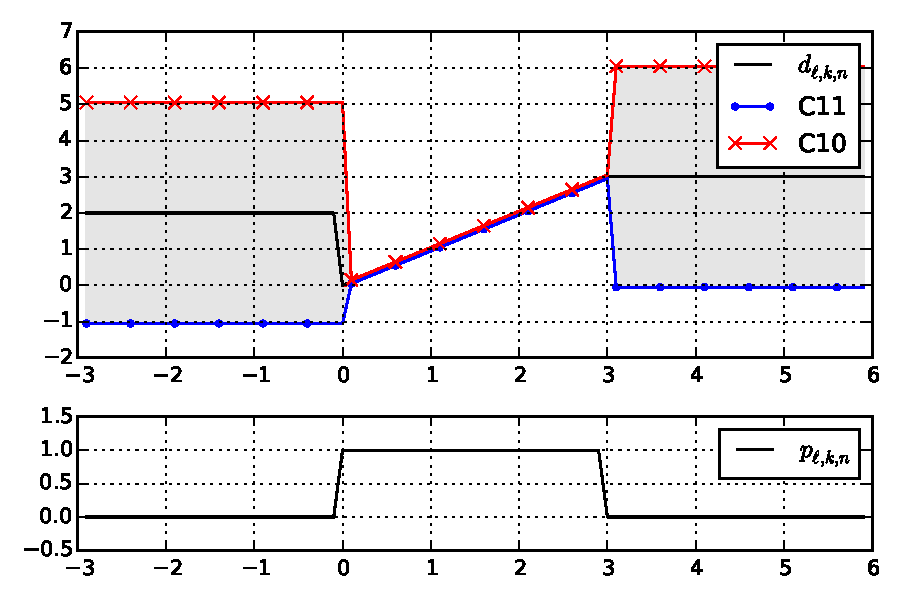
\includegraphics[width=0.45\textwidth]{phase_plot_fig_1.pdf}}
%\subfigure[]{
%\label{fig:pd:inactive}
%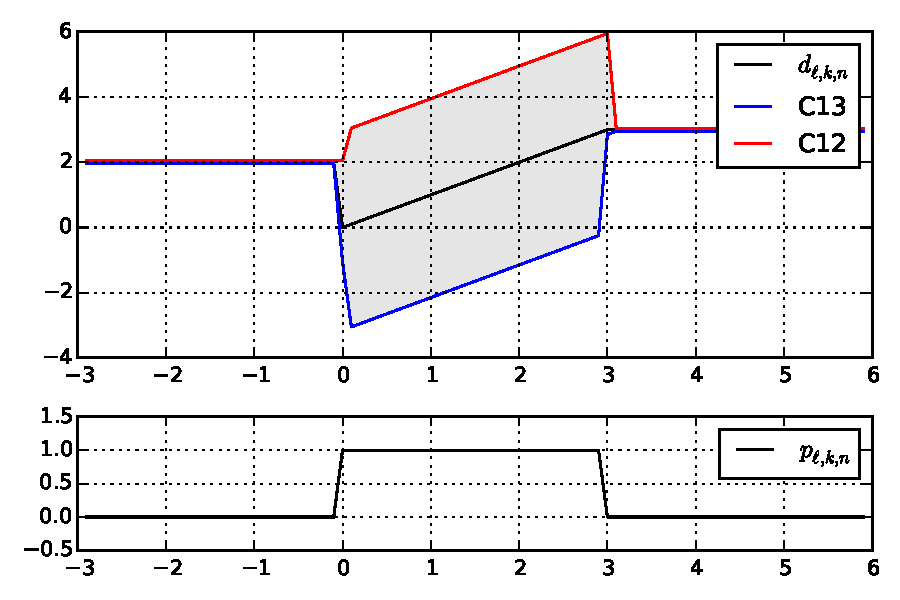
\includegraphics[width=0.45\textwidth]{phase_plot_fig_2.pdf}}
%\subfigure[]{
%\label{fig:pd:resetAndLB}
%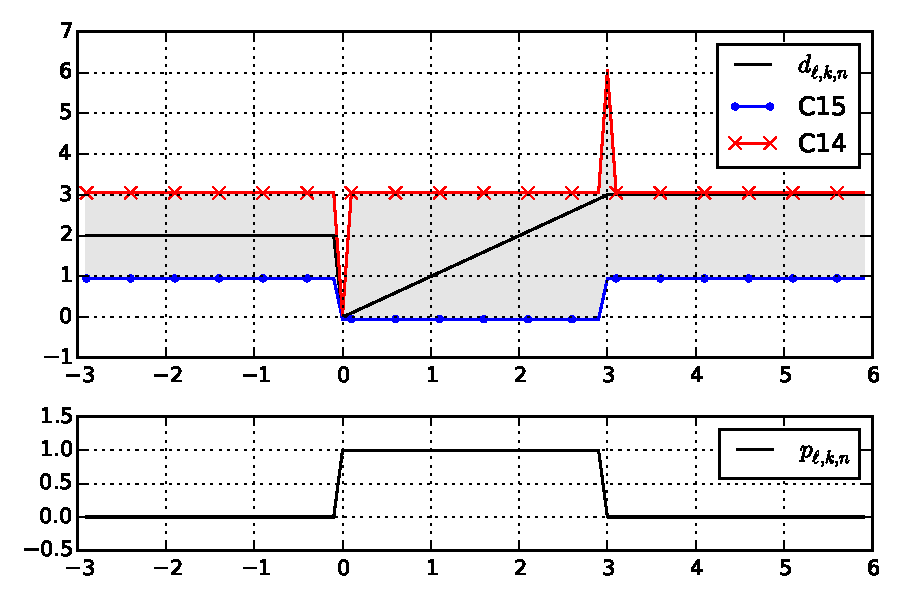
\includegraphics[width=0.45\textwidth]{phase_plot_fig_3.pdf}}
%\subfigure[]{
%\label{fig:cycleTimeC}
%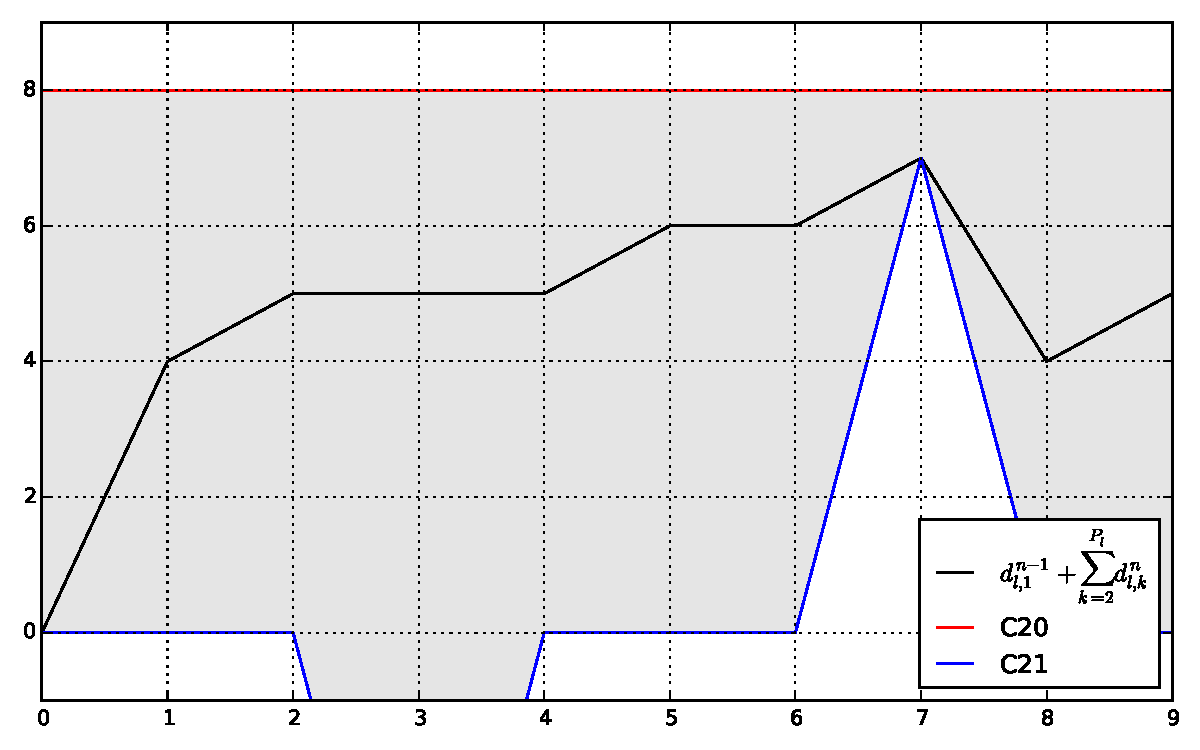
\includegraphics[width=0.45\textwidth]{phase_plot_fig_4.pdf}}
%%
%\caption{Visualization of constraints (\ref{c:pd:incUB}--\ref{c:cycleUB})
%for a traffic light \tl as a function of time.
%%
%(a--c) present, pairwise, the constraints (\ref{c:pd:incUB}--\ref{c:minPhase})
%for phase $k$ (\pd{\ell}{k} as the black line) and the activation variable
%\p[n]{\ell}{k} in the small plot.
%%
%(d) presents the constraints for the cycle time of \tl (\ref{c:cycleLB} and
%\ref{c:cycleUB}), where T.C.T. is the total cycle time and is the left hand side
%of both constraints.
%%
%For this example, $\PTMIN{\ell}{k}=1$, $\PTMAX{\ell}{k}=3$, $\CTMIN{\ell}=7$, and
%$\CTMAX{\ell}=8$.}
%\label{fig:phase_plots}
%\end{figure*}



Next, we enforce the minimum and maximum phase durations (i.e.,
$\PTMIN{\ell}{k}$ and $\PTMAX{\ell}{k}$) for each phase $k \in \Pset_\tl$ of
traffic light \tl.
%
To encode these constraints, we use the helper variable $\pd{\ell}{k} \in
[0,\PTMAX{\ell}{k}]$, defined by constraints
(\ref{c:pd:incUB}--\ref{c:pd:reset}), that:
%
(i) holds the elapsed time since the start of phase $k$ when $\p[n]{\ell}{k}$ is
active~(\ref{c:pd:incUB},\ref{c:pd:incLB});
%
(ii) is constant and holds the duration of the last phase until the next
activation when $\p[n]{\ell}{k}$ is
inactive~(\ref{c:pd:inactiveUB},\ref{c:pd:inactiveLB}); and
%
(iii) is restarted when phase~$k$ changes from inactive to
active~\eqref{c:pd:reset}.
%
Notice that (\ref{c:pd:incUB}--\ref{c:pd:reset}) employs the \textit{big-M}
method to turn the cases that should not be active into subsumed constraints
based on the value of $\p[n]{\tl}{k}$.
%
We use~\PTMAX{\ell}{k} as our large constant since $\pd[n]{\ell}{k} \le
\PTMAX{\ell}{k}$ and $\DT[n] \le \PTMAX{\ell}{k}$.
%
Similarly, \cref{c:minPhase} ensures the minimum phase time of $k$ and is
not enforced while $k$ is still active.
%
%Figures (fig:pd:inc,fig:pd:inactive,fig:pd:resetAndLB) present an example of how
%(\ref{c:pd:incUB}--\ref{c:minPhase}) work together as a function of the time $n$ 
%for $\pd[n]{\ell}{k}$; the domain constraint $0 \le \pd[n]{\ell}{k} \le
%\PTMAX{\ell}{k}$ for all $n \in \{1,\dots,\Nn\}$ is omitted for clarity.
%
%% FWT: I think the mathematical definition of \pd is redundant now.
%\begin{equation}
%\pd{\ell}{k} = 
%\begin{cases}
%\pd[n-1]{\ell}{k} + \DT[n-1] & \p[n-1]{\ell}{k}=1,\p{\ell}{k}=1\\
%\pd[n-1]{\ell}{k} & \p{\ell}{k}=0\\
%0 & \p[n-1]{\ell}{k}=0,\p{\ell}{k}=1
%\end{cases}
%\label{def:pd}
%\end{equation}
%
%% TODO(fwt): I believe that that \pd{\ell}{k} (above) could be redefined by
%% shifting it by delta_n resulting in a d_{l,k,n} representing the total time
%% until the end of interval **n** instead of n-1. This would be more intuitive
%% and would simplify c:cycleLB and c:cycleUB. This is what I propose:
%% d_{l,k,n} = d_{l,k,n-1} + delta-t_{n}  if p_{l,k,n-1} = p_{l,k,n} = 1
%%           = d_{l,k,n-1}                if p_{l,k,n} = 0
%%           = delta-t_{n}                if p_{l,k,n-1} 0 and p_{l,k,n} = 1
%
%% FWT: this constraint is define as the variable domain
%\pd{\ell}{k} &\le \PTMAX{\ell}{k}\tag{C19}\label{eq:C19}\\
%
\begin{cAlign}
%
\pd{\ell}{k} &\le
  \pd[n-1]{\ell}{k} + \DT[n-1] \p[n-1]{\ell}{k} 
  + \PTMAX{\ell}{k} (1 - \p[n-1]{\ell}{k})\tagconstrain{c:pd:incUB}\\
%
\pd{\ell}{k} &\ge
  \pd[n-1]{\ell}{k} + \DT[n-1] \p[n-1]{\ell}{k}
  - \PTMAX{\ell}{k} (1 - \p[n-1]{\ell}{k})\tagconstrain{c:pd:incLB}\\
%
\pd{\ell}{k} &\le \pd[n-1]{\ell}{k} + \PTMAX{\ell}{k} \p[n-1]{\ell}{k}
  \tagconstrain{c:pd:inactiveUB}\\
\pd{\ell}{k} &\ge \pd[n-1]{\ell}{k} - \PTMAX{\ell}{k} \p{\ell}{k}
  \tagconstrain{c:pd:inactiveLB}\\
%\end{cAlign}
%%
%\begin{cAlign}
%%
\pd{\ell}{k} &\le \PTMAX{\ell}{k}(1 - \p{\ell}{k} + \p[n-1]{\ell}{k})
  \tagconstrain{c:pd:reset}\\
%
\pd{\ell}{k} &\ge \PTMIN{\ell}{k}(1 - \p{\ell}{k}) \tagconstrain{c:minPhase}
%
\end{cAlign}
%


Lastly, we constrain the sum of all the phase durations for light \tl to be
within the cycle time limits \CTMIN{\tl}~\eqref{c:cycleLB} and
\CTMAX{\tl}~\eqref{c:cycleUB}.
%
In both \eqref{c:cycleLB} and \eqref{c:cycleUB}, we use the duration of phase 1
of \tl from the previous interval $n-1$ instead of the current interval $n$
because \eqref{c:pd:reset} forces \pd[n]{\tl}{1} to be 0 at the beginning of
each cycle;
%
however, from the previous end of phase 1 until $n-1$, \pd[n-1]{\tl}{1} holds
the correct elapse time of phase 1.
%
Additionally, \eqref{c:cycleLB} is enforced right after the end of the each
cycle, i.e., when its first phase is changed from inactive to active.
%
%%The value \eqref{c:cycleLB} and \eqref{c:cycleUB} over time for a traffic light
%%\tl is illustrated in Figure (fig:cycleTimeC).
%
\begin{cAlign}
%
\pd[n-1]{\ell}{1} + \sum\limits_{k=2}^{\Pn} \pd{\ell}{k} &\ge \CTMIN{\ell}
(\p{k}{1} - \p[n-1]{k}{1}) \tagconstrain{c:cycleLB}\\
%
\pd[n-1]{\ell}{1} + \sum\limits_{k=2}^{\Pn} \pd{\ell}{k} &\le \CTMAX{\ell}
\tagconstrain{c:cycleUB}
%
\end{cAlign}
%
The MILP~(\ref{eq:objFunc},~\ref{c:turnProb}--\ref{c:cycleUB}) encodes
the problem of finding the optimized adaptive traffic control
plan in a QTM network without light rail.

\paragraph{Light Rail Constraints}
%
To incorporate a fixed-schedule light rail in our model, we post-process our
MILP model by fixing the free variable $\p[n]{\tl}{k}$ for all $n$ such that the
light rail uses phase $k$ of \tl at time $n$.
%
Formally, given a schedule $S_{\tl}(k,n) \in \{0,1\}$ where~$1$ represents that
the light rail uses phase $k$ of \tl at time $n$, we replace
(\ref{c:pd:incUB}--\ref{c:minPhase}) by \eqref{c:forceTransit} and
\eqref{c:pd:holdTransit} when $\sum_{k \in \Pset_\tl} S_{\tl}(k,n) > 0$.
%
%\begin{cAlign}
%%
%\p[n]{\ell}{k} &= S_{\ell}(k,n)\tagconstrain{c:forceTransit}\\
%%
%\pd{\ell}{k} &= \pd[n-1]{\ell}{k}\tagconstrain{c:pd:holdTransit}
%%
%\end{cAlign} \noindent\begin{minipage}{0.5\linewidth}
\begin{cAlign} 
%
\p[n]{\ell}{k} &= S_{\ell}(k,n)\tagconstrain{c:forceTransit}\\
%
%\end{cAlign} \end{minipage}% \begin{minipage}{0.5\linewidth} \begin{cAlign} 
%
\pd{\ell}{k} &= \pd[n-1]{\ell}{k}\tagconstrain{c:pd:holdTransit}
%
\end{cAlign}
%\end{minipage}\par\vspace{\belowdisplayskip}
%
\noindent \eqref{c:forceTransit} enforces that the correct phase $k$ is active
when the light rail reaches the traffic light $l$, and
%
%the effect of \eqref{c:pd:holdTransit} is to not count the time used by the
%light rail towards the total duration of the phase $k$.
%
\eqref{c:pd:holdTransit} ensures that the light rail can pass through $l$ even
if more than the maximum phase time \PTMAX{\tl}{k} is necessary.


\subsection{QTM as a Fixed-Time Controller}

We can further extend QTM to compute an optimized control plan with fixed phase
durations.
%
For all~$\tl \in \Lset$, $k \in \Pset_\tl$, we introduce the new variable
$\PTFIXED{\ell}{k} \in [\PTMIN{\ell}{k}, \PTMAX{\ell}{k}]$ and replace the
bounds constraints on $\pd[n]{\ell}{k}$ (that is, $\pd[n]{\ell}{k} \le
\PTMAX{\ell}{k}$ and \ref{c:minPhase}) with fixed the duration
constraints~(\ref{c:pd:fixedUB}-\ref{c:pd:fixedLB}).
%
\begin{cAlign} \pd{\ell}{k} &\le \PTFIXED{\ell}{k} + \PTMAX{\ell}{k}
  \p[n]{\ell}{k} \tagconstrain{c:pd:fixedUB}\\
%
  \pd{\ell}{k} &\ge \PTFIXED{\ell}{k} - \PTMAX{\ell}{k} \p[n]{\ell}{k}
  \tagconstrain{c:pd:fixedLB} \end{cAlign}


Similarly to the variable phase duration constraints, the \textit{big-M} method
is employed to enforce (\ref{c:pd:fixedUB}-\ref{c:pd:fixedLB}) only while the
phase is inactive.
%
Furthermore, these constraints are only applied over time intervals $n$ such
that $\tn[n] > \CTMAX{\tl}$ in order to allow the controller to optimize an
initial phase offset at the start of the plan.
%TODO talk about how the fixed phase times fit around transit crossings.



%To incorporate a fixed-schedule light rail in our model, we enforce phase $k$ used
%by the light rail is always on when the transit crosses at light \tl, i.e., we add
%the constraint $\p[n]{\ell}{k} = 1$ for all $n$ s.t.\ the light rail uses phase $k$
%of \tl at time $n$.
%%
%%
%We also hold $\pd{\ell}{k}$ constant while the light rail crosses \tl, i.e., 
%$\pd{\ell}{k} = \pd[n-1]{\ell}{k}$.
%%
%Since the light rail schedule is fixed and known a priori, adding these extra
%constraints are done in a preprocessing phase before the MILP is solved.
